 \documentclass[a4paper, 10pt, final]{article}

\usepackage{a4wide}

\usepackage{charter}
\usepackage{verbatim}
\usepackage{amsfonts}
\usepackage{amsmath}
\usepackage{amsthm}
\usepackage{amssymb}
%\usepackage[integrals]{wasysym}
%\usepackage{mathrsfs}
%\usepackage[mathcal]{euscript}
\usepackage{listings}
\usepackage{graphicx}
\usepackage{multirow}
\usepackage{hyperref}
\usepackage{float}
\usepackage[small,bf]{caption}
%\usepackage{xypic}
\usepackage[table]{xcolor}
\usepackage{subfig}
%\usepackage{ulem} %use \normalem after begin document
\usepackage[authoryear]{natbib}

% Settings
\parindent=5pt
\parskip=8pt plus 2pt minus 4pt
\lstset{language=Matlab, basicstyle=\scriptsize,
    showstringspaces=false, numbers=left, stepnumber=1, numberstyle=\tiny, frame=tb}


%% \def\mytitle{Signal and Image Processing 2010}
%% \def\mysubtitle{Handin of mandatory excercise 1}
%% \def\myauthor{Ulrik Bonde}
%% \def\mymail{\mailto{bonde@diku.dk}}
%% \def\mydate{\today}

\title{Statistical Methods for Machine Learning \\ Mandatory Project 2}
\author{Kasper Steenstrup\\Michael Andersen\\Esben Skaarup}
\date{\today}

%% \title{\mytitle}
%% \subtitle{\mysubtitle}

%% \author{\myauthor{} - \mymail}
%% \date{\mydate}

\hypersetup{
colorlinks,%
citecolor=black,%
filecolor=black,%
linkcolor=black,%
urlcolor=black,%
bookmarksopen=false,
pdftitle={Statistical Methods for Machine Learning - Mandatory Project 2},
pdfauthor={Kasper Steenstrup, Michael Andersen \& Esben Skaarup}
}

\begin{document}
\maketitle

\subsection*{Question 2.1}
\subsection*{Question 2.1}

We calculate the RMS error for the two models, this is displayed in
table \ref{tab:q21} along with the min and max averaged over 50
iterations. In the first model the RMS error is lower than the other,
the first model min and max is also closer. Based on this fact, we see
that the first model is better, this was to be expected as the first
model is based on four features from the dataset and the second model
is based on one features from the dataset.

\begin{table}[!htbp]
  \centering
  \begin{tabular}{| l | l | l | l |}
    \hline
    {}		& RMS		& Max		& Min \\
    \hline
    Train1	& 4.4071	& 4.5634	& 4.2075 \\
    \hline
    Test1	& 4.5723	& 5.3269	& 3.9773 \\
    \hline
    Train2	& 4.8466	& 5.0046	& 4.5746 \\
    \hline
    Test2	& 4.9268	& 6.0025	& 4.2679 \\
    \hline
  \end{tabular}
  \caption{Shows the Root mean square, along with maximum and minimum.}
  \label{tab:q21}
\end{table}

\newpage


\subsection*{Question 2.2}
\subsection*{Question 2.2}
In figure \ref{fig:q22} the four RMS errors for $\alpha$ in the
interval from 1--200. As the figure indicates the test data, have the
lowest error, and the firste model have the best results, due to the
fact that it uses more features from the dataset to train the
model. The best value of $\alpha$ is one, since the error get bigger
the larger $\alpha$.

\begin{figure}[!htbp]
  \centering
  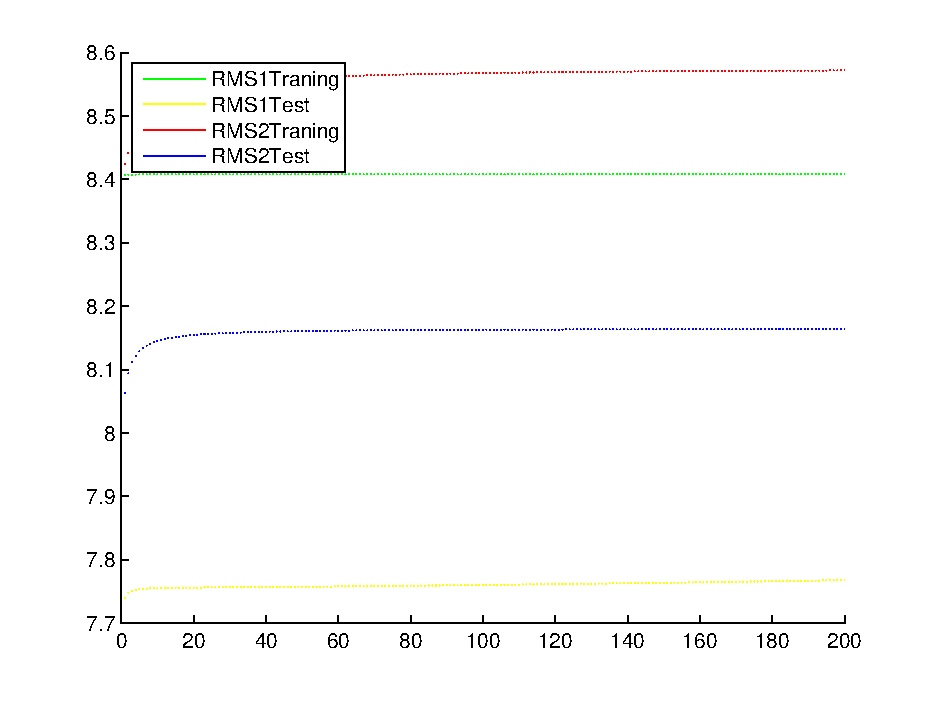
\includegraphics[width=0.75\textwidth]{./images/Q2.pdf}
  \caption{RMS for the two training models and test models}
  \label{fig:q22}
\end{figure}




%%%%%%%%%%%%%%%%%%%%%%%%%%%%%%%%%%%%%%%%%%%%%%%%%%%%%%%%%%%%%%%%%%%%
% Formal stuff

%\bibliographystyle{abbrvnat}
%\bibliography{bibliography}
%\addcontentsline{toc}{chapter}{Litteratur

\end{document}

% vim: set tw=72 spell spelllang=en:
